\documentclass[tikz, border=4pt]{standalone}
\usepackage{amsmath}
\usepackage{pgfplots}
\pgfplotsset{compat=1.18}
\usetikzlibrary{pgfplots.groupplots}

\begin{document}
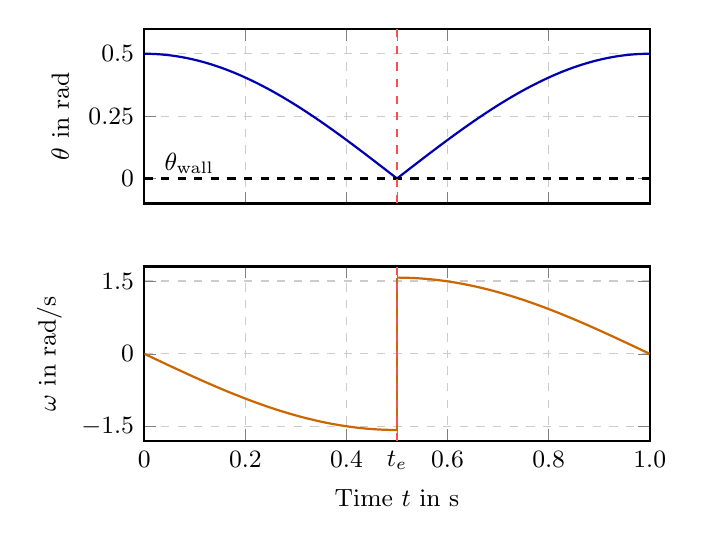
\begin{tikzpicture}
\begin{groupplot}[
    group style={
        group size=1 by 2,
        vertical sep=0.8cm,
        x descriptions at=edge bottom,
    },
    width=8cm, height=3.8cm,
    xmin=0, xmax=1.0,
    xtick={0, 0.2, 0.4, 0.5, 0.6, 0.8, 1.0},
    xticklabels={$0$, $0.2$, $0.4$, $t_e$, $0.6$, $0.8$, $1.0$},
    tick align=inside,
    grid=both,
    grid style={dashed, gray!40},
    every axis/.append style={font=\small, line width=0.8pt},
]

%% Panel 1: theta(t) — kink at t_e, position continuous
\nextgroupplot[
    ylabel={$\theta$ in rad},
    ymin=-0.1, ymax=0.6,
    ytick={0, 0.25, 0.5},
]
\addplot[thick, blue!70!black, domain=0:0.5, samples=60]
    { 0.5 * cos(deg(pi * x)) };
\addplot[thick, blue!70!black, domain=0.5:1.0, samples=60]
    { 0.5 * cos(deg(pi * (1.0 - x))) };
\addplot[dashed, black, thick, domain=0:1.0] {0};
\node[right, font=\small] at (axis cs:0.02, 0.06) {$\theta_\text{wall}$};
\addplot[dashed, red!70, thick] coordinates {(0.5, -0.1) (0.5, 0.6)};

%% Panel 2: omega(t) — jump at t_e, velocity discontinuous
\nextgroupplot[
    ylabel={$\omega$ in rad/s},
    xlabel={Time $t$ in s},
    ymin=-1.8, ymax=1.8,
    ytick={-1.5, 0, 1.5},
]
\addplot[thick, orange!80!black, domain=0:0.5, samples=60]
    { -1.57 * sin(deg(pi * x)) };
\addplot[thick, orange!80!black, domain=0.5:1.0, samples=60]
    { 1.57 * sin(deg(pi * (1.0 - x))) };
% vertical jump segment: literal values only
\addplot[thick, orange!80!black] coordinates {(0.5, -1.57) (0.5, 1.57)};
\addplot[dashed, red!70, thick] coordinates {(0.5, -1.8) (0.5, 1.8)};

\end{groupplot}
\end{tikzpicture}
\end{document}
